% "Станет проще"

\documentclass[a4paper,12pt]{article} % тип документа

% report, book

%  Русский язык

\usepackage[T2A]{fontenc}			% кодировка
\usepackage[utf8]{inputenc}			% кодировка исходного текста
\usepackage{graphicx}
\usepackage[english,russian]{babel}	% локализация и переносы


%отступ
\usepackage[left=3cm,right=3cm,
    top=3cm,bottom=3cm,bindingoffset=0cm]{geometry}

% Математика
\usepackage{amsmath,amsfonts,amssymb,amsthm,mathtools} 
\usepackage{csvsimple}
\usepackage{multirow}

\usepackage{hyperref}
\usepackage{wasysym}
\usepackage{subcaption}
\usepackage{verbatim}
\usepackage{hyperref}
\usepackage{float}
\usepackage{enumerate}
\usepackage[dvipsnames]{xcolor}
%Заговолок
%\graphicspath{ {images/} }
\graphicspath{ {img/} }

\begin{titlepage}
\author{Соловьянов Михаил }
\title{Задание 28. Термодинамика (ЕГЭ)}
\date{\today}
\end{titlepage}



\begin{document} % начало документа
\maketitle



\section{Задачи}


\subsection{•}

\begin{figure}[H]
\centering
  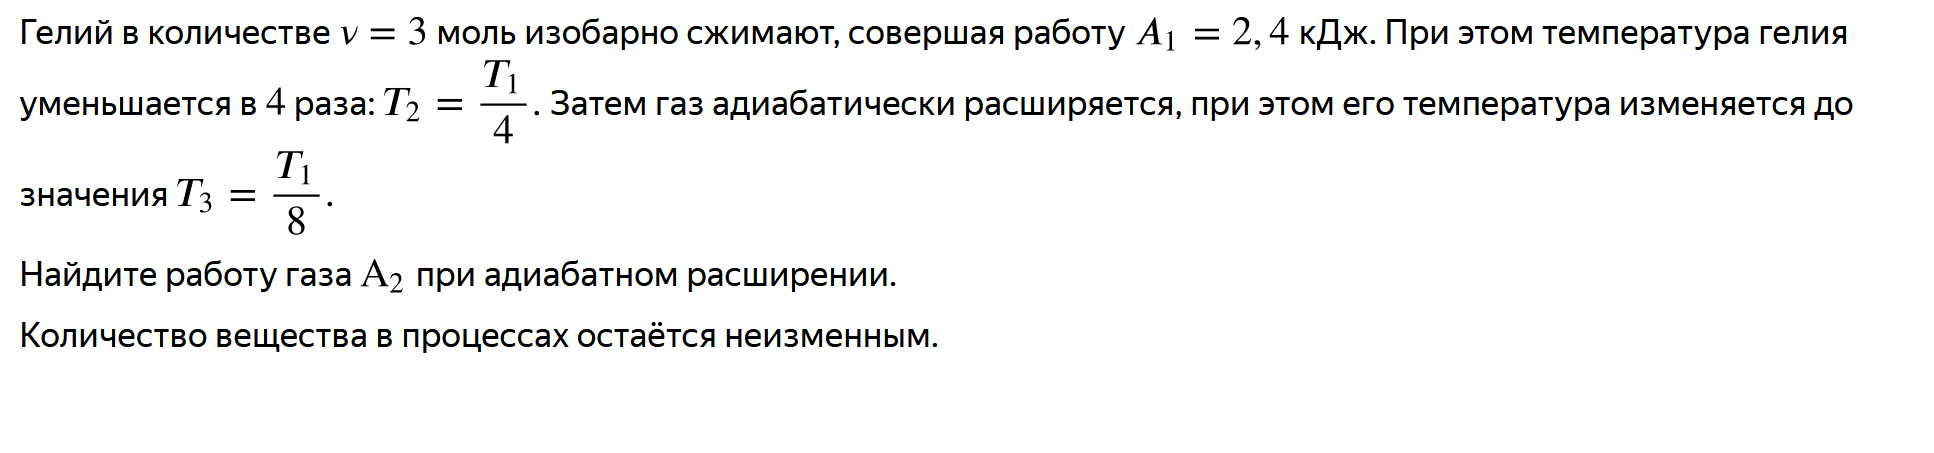
\includegraphics[width=1.1\linewidth]{1.PNG}
  % \caption{Задача 1}
  \label{task0}
\end{figure}

\subsection{•}

\begin{figure}[H]
\centering
  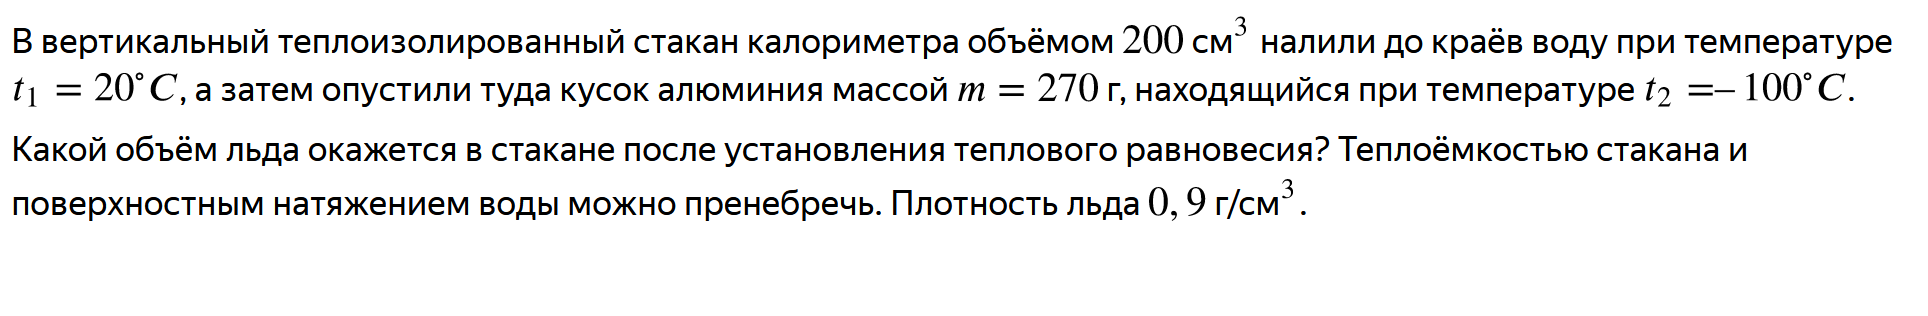
\includegraphics[width=1.1\linewidth]{2.PNG}
  %\caption{Задача 2}
  \label{task2}
\end{figure}

\subsection{•}

\begin{figure}[H]
\centering
  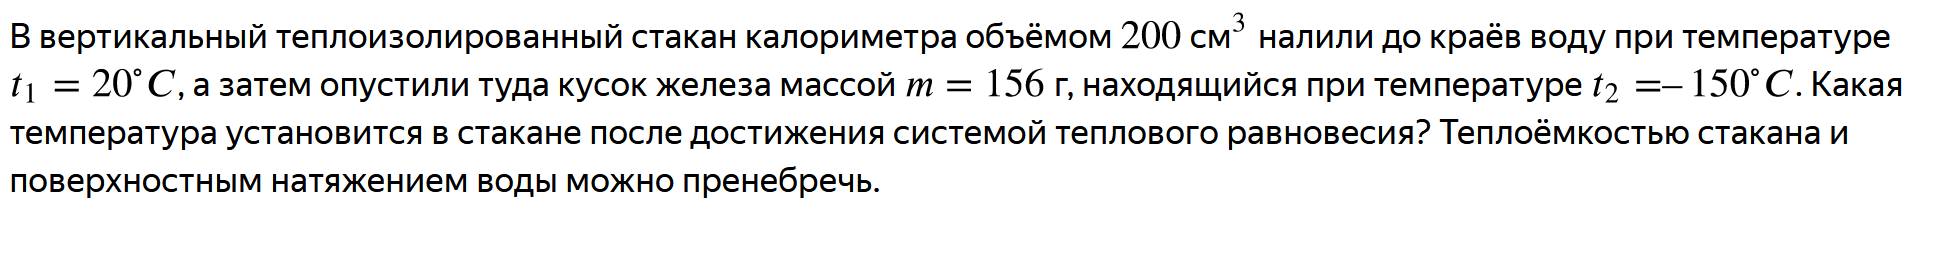
\includegraphics[width=1.1\linewidth]{3.PNG}
  %\caption{Задача 2}
  \label{task2}
\end{figure}

\subsection{•}

\begin{figure}[H]
\centering
  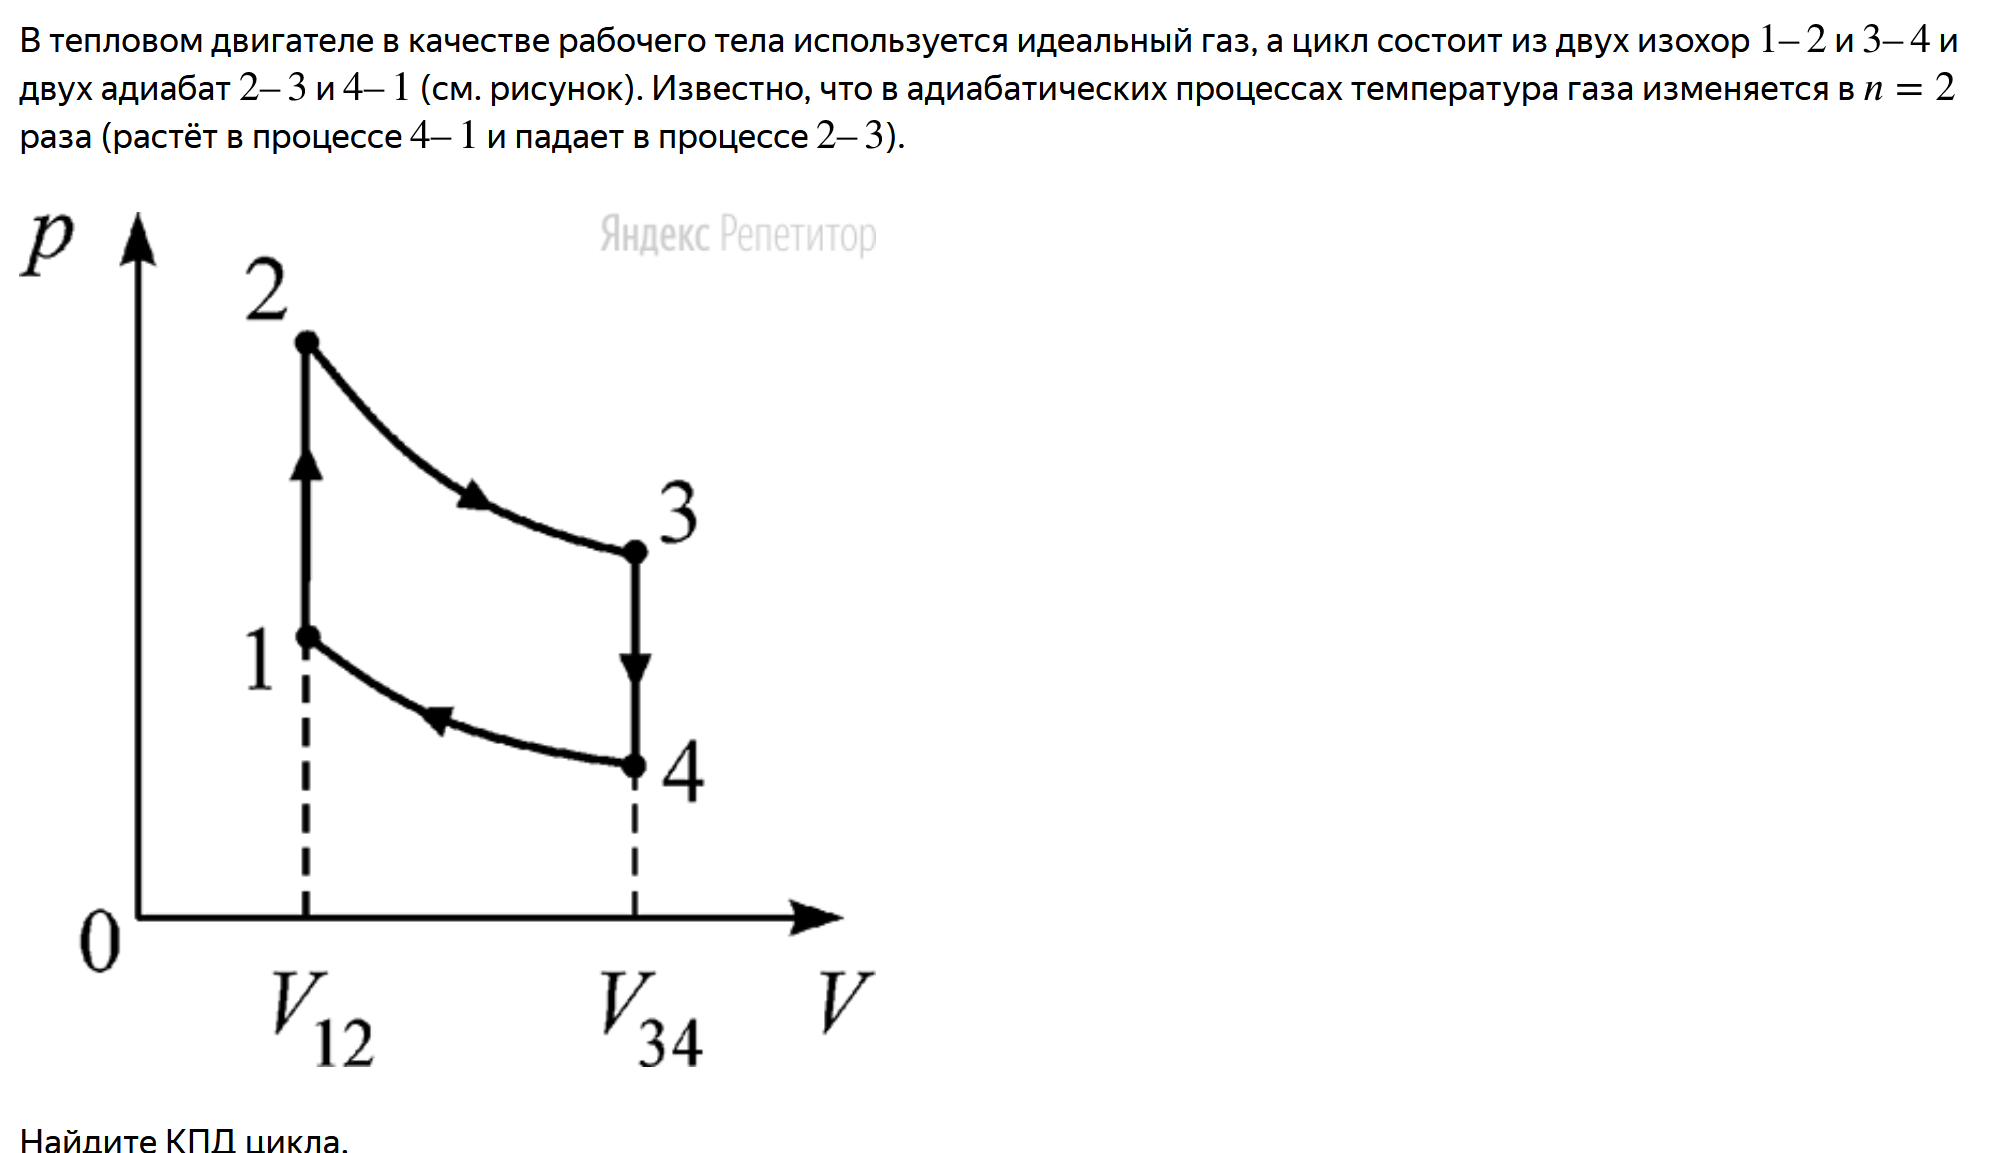
\includegraphics[width=1.1\linewidth]{4.PNG}
  %\caption{Задача 2}
  \label{task2}
\end{figure}

\subsection{•}

\begin{figure}[H]
\centering
  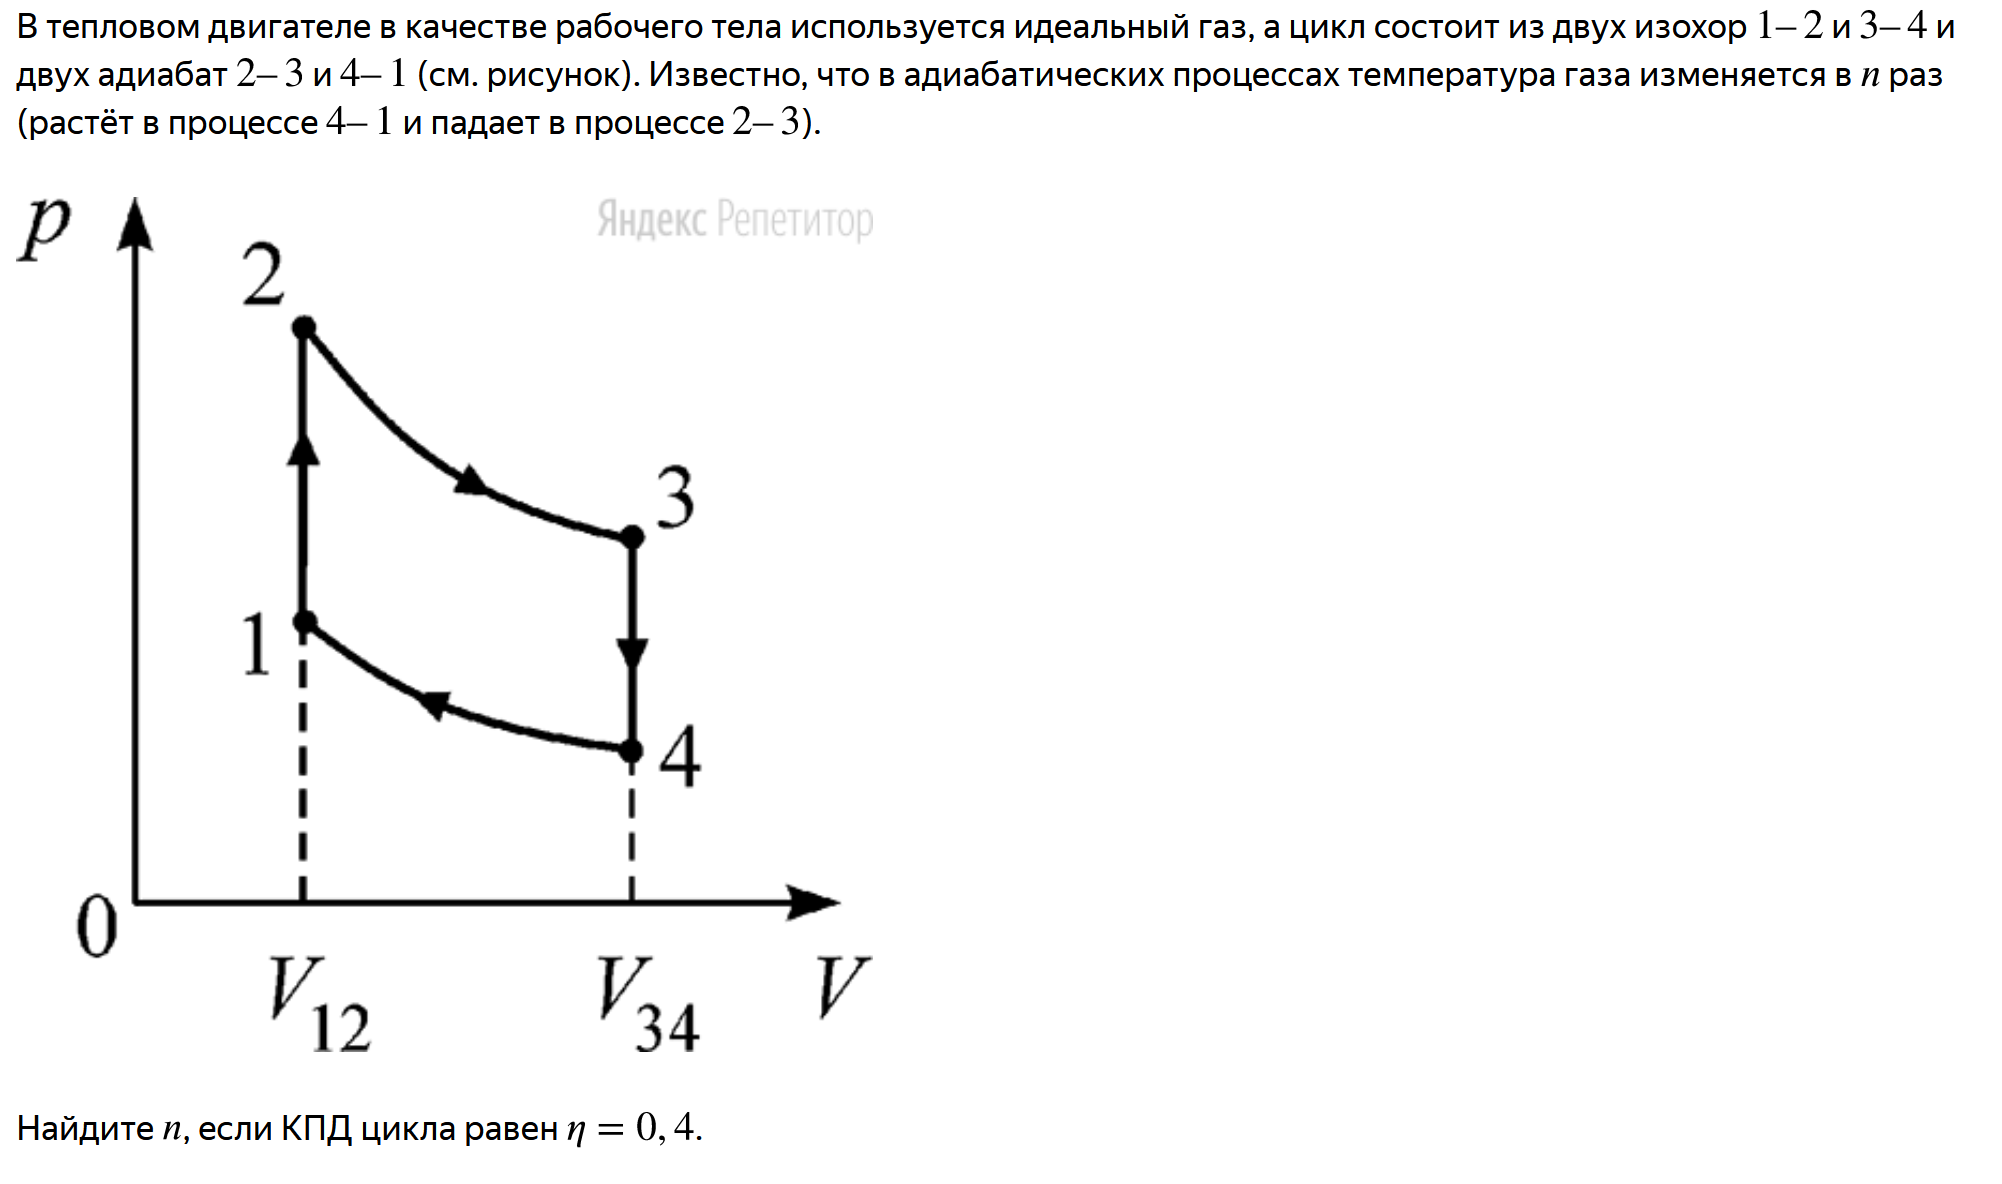
\includegraphics[width=1.1\linewidth]{5.PNG}
  %\caption{Задача 2}
  \label{task2}
\end{figure}


\subsection{•}

\begin{figure}[H]
\centering
  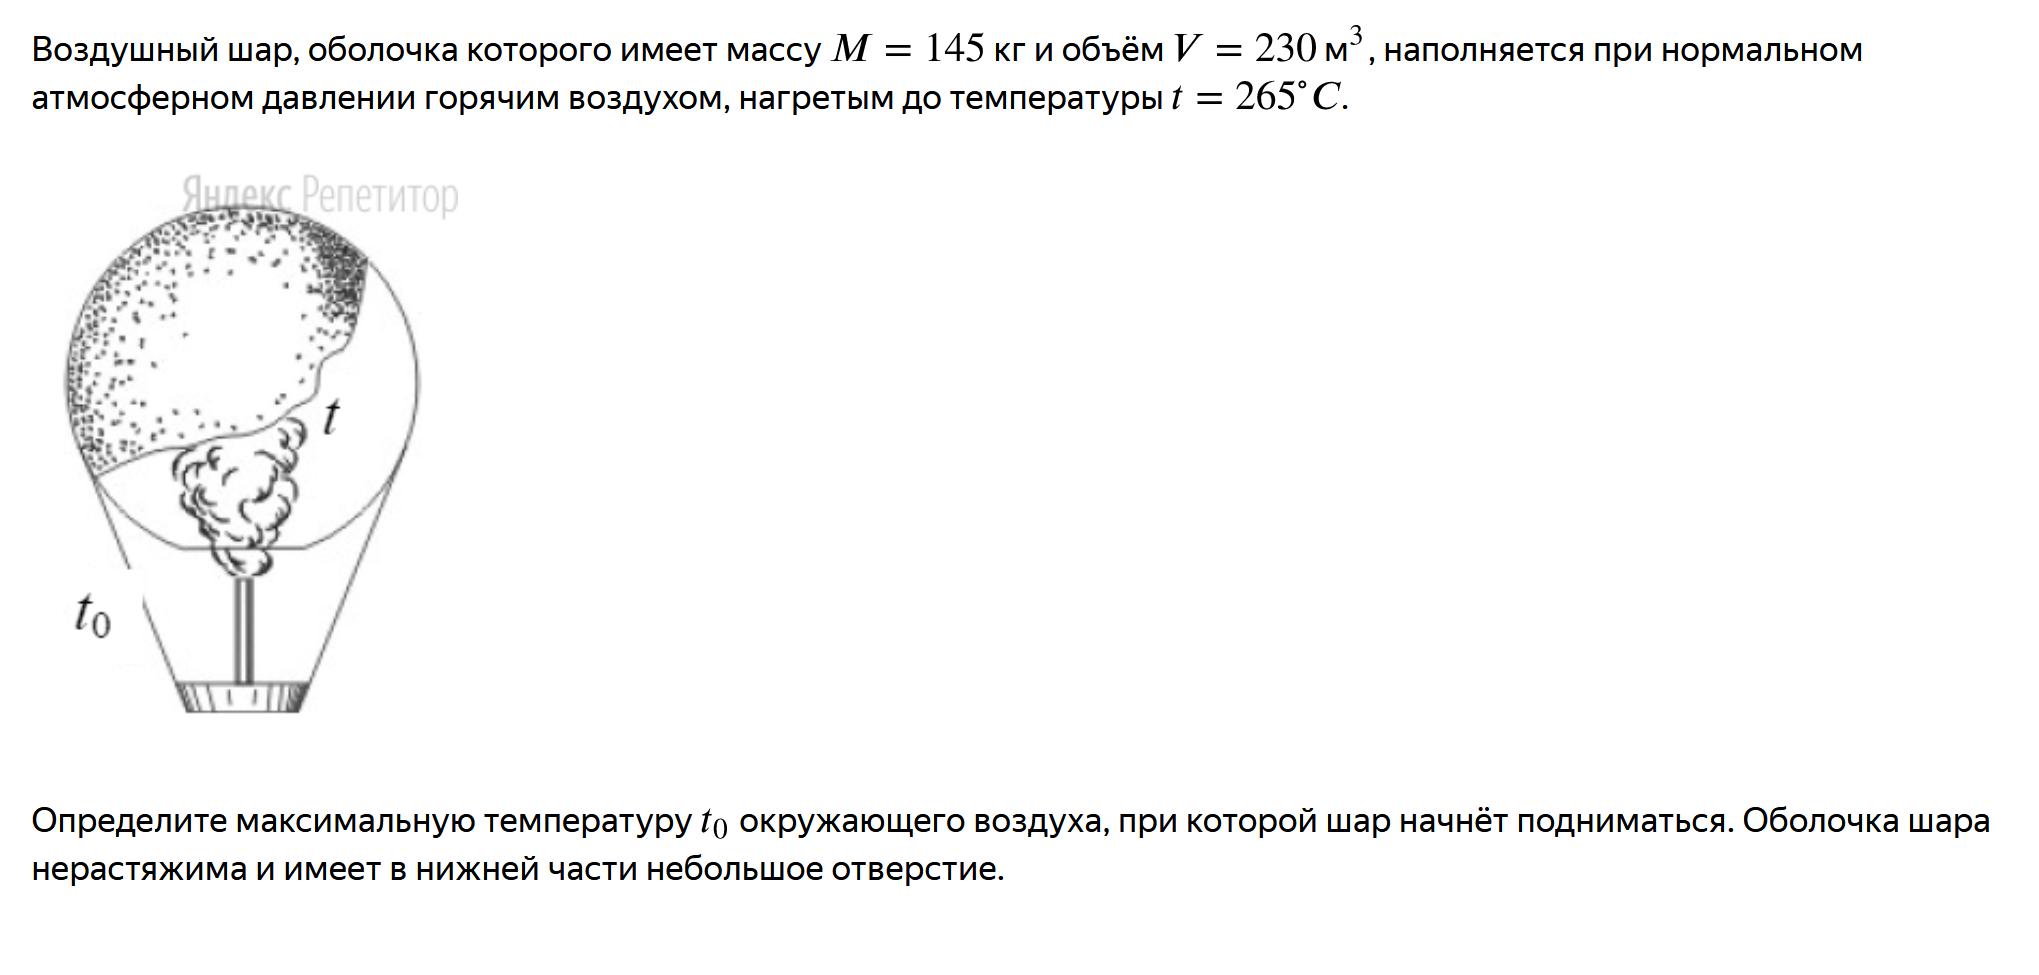
\includegraphics[width=1.1\linewidth]{6.PNG}
  %\caption{Задача 2}
  \label{task2}
\end{figure}


\section{Вариант ЕГЭ}
\colorbox{Red}{Решить вариант ЕГЭ по адресу:}
 \\ \textit{(./fiz-v1.pdf)} (в этой папке)


\end{document}